\documentclass[12,a4paper]{article}
\usepackage{fontspec}
\usepackage{geometry}
\usepackage{fontspec}
\usepackage{xeCJK}
\usepackage{amsmath}
\usepackage{fancyhdr}
\usepackage{physics}
\usepackage{tikz}
\usepackage{graphicx}
\usepackage{placeins}
\usetikzlibrary{positioning}
\setCJKmainfont{標楷體}
\XeTeXlinebreaklocale "zh"
\XeTeXlinebreakskip = 0pt plus 1pt
\geometry{a4paper,scale=0.8}
\pagestyle{fancy}
\fancyhf{}
\rhead{Artificial-Intelligence}
\lhead{張紳濡}
\cfoot{\thepage}
\title{{\Huge Artificial-Intelligence} \\ homework1 }
\author{0816023 張紳濡}
\date{}
\begin{document}
\maketitle
\thispagestyle{fancy}
\section{Introduction}
使用Adaboost與Yolov5對停車場的車輛進行偵測。
\section{Data}
\begin{itemize}
\item train: \tx{600 car pictures and 600 non-car pictures.}
\item test: \tx{600 car pictures and 600 non-car pictures.}
\item detect: \tx{A gif video with 50 pictures.}
\end{itemize}
\section{Adaboost Algorithm}
使用許多WeekClassifier組合起來,每次做完調整weight使當前的error rate達到0.5並將新的weight傳遞給下個WeekClassifier(這部分在adaboost.py train function內已寫好,詳細不在這贅述)
\begin{figure}[!ht]
\centering
\includegraphics[width=0.8\textwidth]{pic/code/pic01.png}
\end{figure}
\section{What I do}
\subsection{Part I Load Data}
將train與test的car, non-car圖片讀進並轉灰階與resize,將其轉成nparray並與label一起包成tuple,存進一個list。
\begin{figure}[!ht]
\centering
\includegraphics[width=0.8\textwidth]{pic/code/pic02.png}
\end{figure}
\subsection{Part II SelectBest}
用features產生一堆WeekClassifier(features大約有13W)
\begin{itemize}
    \item feature:
    \begin{itemize}
        \item \tx{line 181: 每次將feature傳進classifier.py內的WeekClassifier,並將threshold設為0}
        \item \tx{line 180: 每次將feature傳進classifier.py內的WeekClassifier,並將threshold設為mean(mean(car\_featureval)$+$mean(non-car\_featureval))}
    \end{itemize}
    \item \tx{將ii傳進去(600張)計算,回傳一個boolean值。}
    \item \tx{對於每次的ii若回傳直不等於其label,將其加入errorsum(line 185)}
    \item \tx{對於每個feature,若其errorsum $<$ mineerror,將minerror更新並將其記錄為bestclf(line 187)。}
    \item \tx{將minerror normalize,設為bestError(line 191)。}
\end{itemize}
\begin{figure}[!ht]
\centering
\includegraphics[width=0.8\textwidth]{pic/code/pic03.png}
\end{figure}
\subsection{Part III Additional experiments}
對於Part II兩種方法,T從0到10進行測試得到以下圖表
\begin{figure}[!ht]
\begin{subfigure}
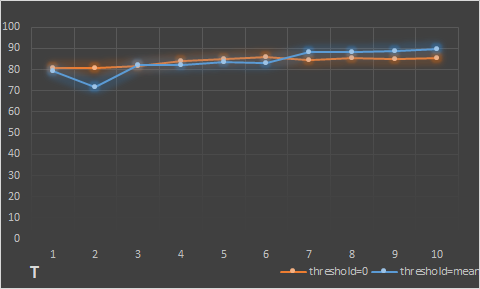
\includegraphics[width=0.5\textwidth]{pic/orignvsmean.png}
\end{subfigure}
\begin{subfigure}
\includegraphics[width=0.5\textwidth]{pic/orignvsmeanval.png}
\end{subfigure}
\end{figure}
\FloatBarrier
兩可以發現兩者在T變大時正確率都會提高,但Threshold = mean在更高的T有更好的表現,最後的比較我拿Threshold =0,T=6與Threshold = mean,T=10來比較
\subsection{Part IV Detect car}
\begin{itemize}
    \item 將video.gif與detectData.txt讀進來(line 59~62)
    \item 對於每張frame使用crop fuction切出360*160的圖片並resize成36*16的圖片轉成灰階(line 72,73)
    \item 傳入Part III訓練好的clf(line 74)
    \item 若回傳值為1就在其對應值畫出四邊形並輸出1或0(line 77~80)
    \item 最後輸出這張畫好的frame(line 88)(這邊我輸出了全部50張frame到code內的路徑)
\end{itemize}
\begin{figure}[!ht]
\centering
\includegraphics[width=0.8\textwidth]{pic/code/pic04.png}
\end{figure}
\FloatBarrier
\subsection{Part V compare with Yolov5}
\subsubsection{三種方法的第一張frame:}
\begin{figure}[!ht]
\centering
    \begin{subfigure}
    \centering
    \caption{Adaboost T = 6,Threshold = 0}
    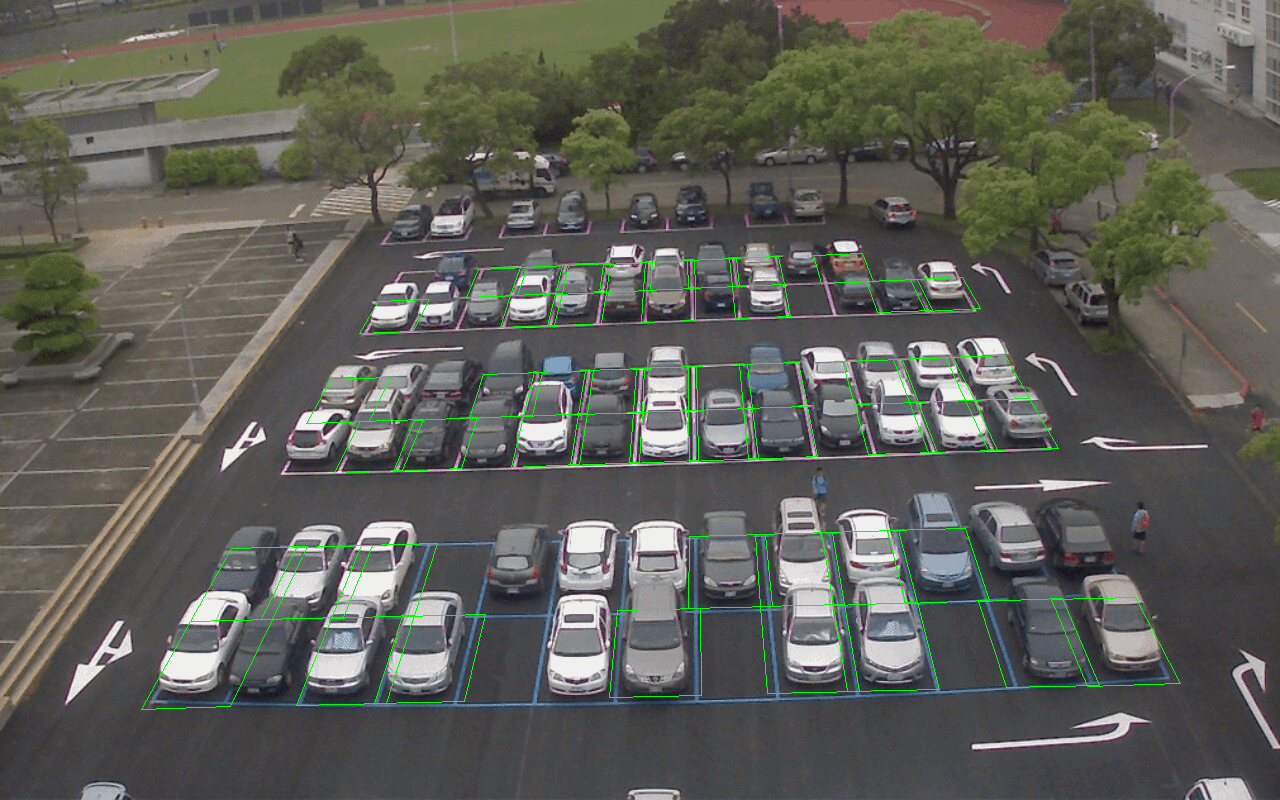
\includegraphics[width=0.5\textwidth]{pic/detectpicorigin/adaboostpic0.png}
    \end{subfigure}
    \begin{subfigure}
    \centering
    \caption{Adaboost T = 10,Threshold = 0}
    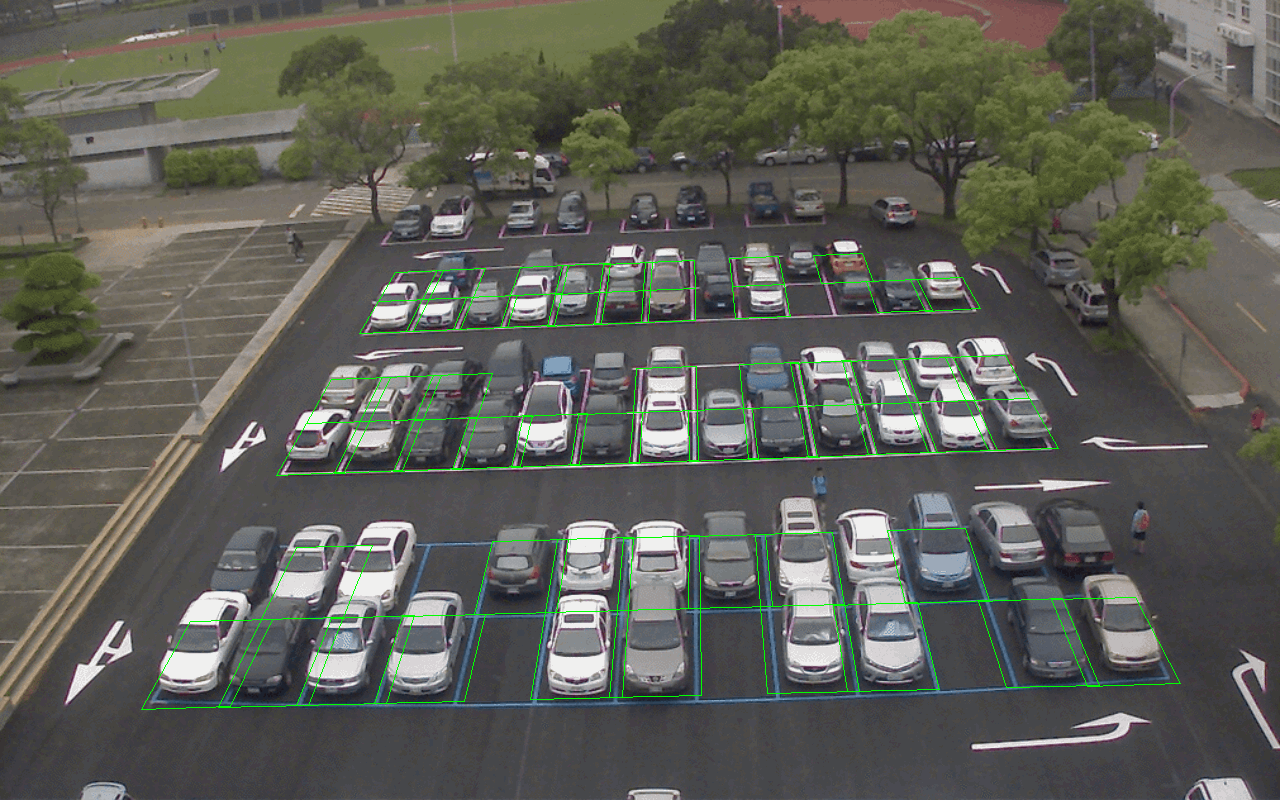
\includegraphics[width=0.5\textwidth]{pic/detectpicm/adaboostpic_m0.png}
    \end{subfigure}
    \begin{subfigure}
    \centering
    \caption{yolov5,confidence = 0.4}
    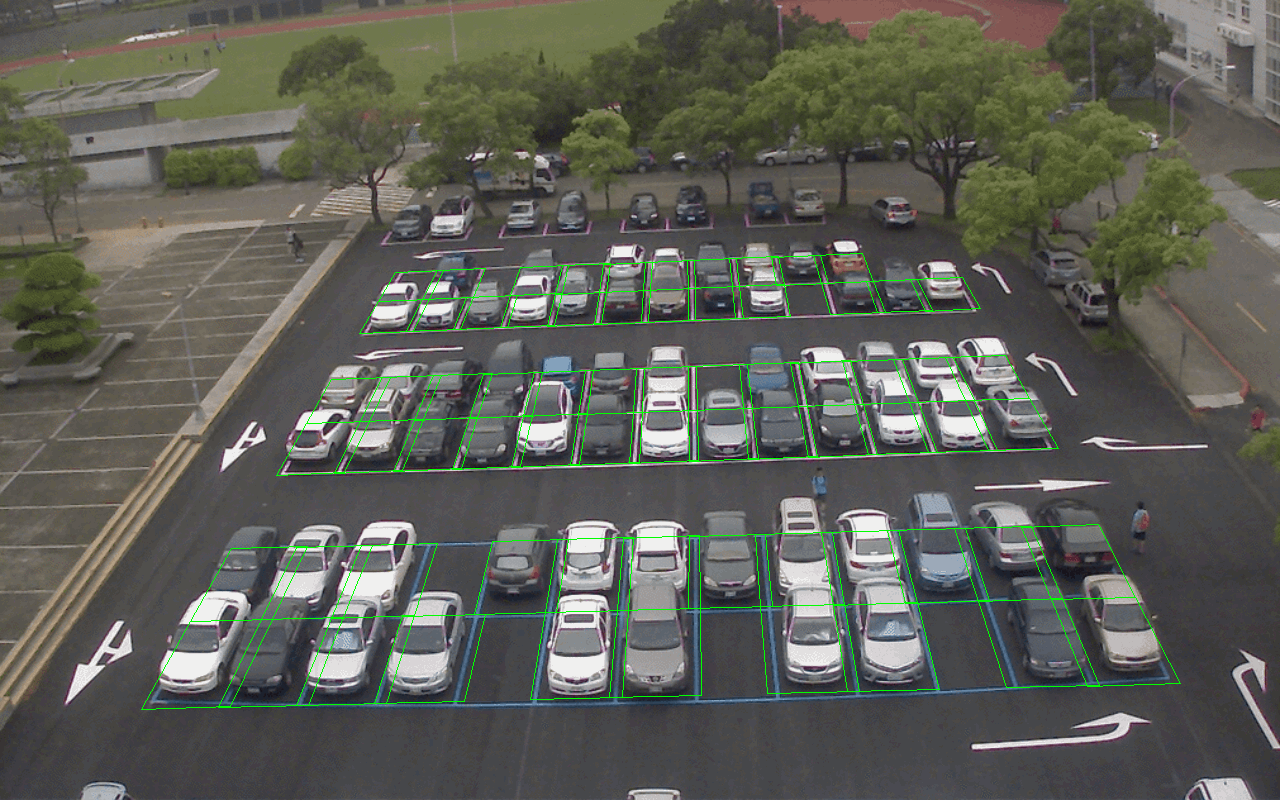
\includegraphics[width=0.5\textwidth]{pic/Yolov5_first_frame.png}
    \end{subfigure}
\end{figure}
\FloatBarrier
\subsubsection{三種方法的Accuracy:}
\begin{figure}[!ht]
    \centering
    \caption{Accuracy}
    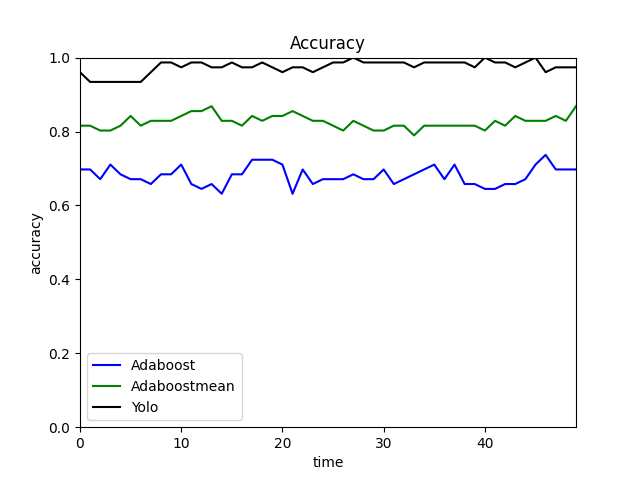
\includegraphics[width=0.5\textwidth]{pic/Accuracy.png}
\end{figure}
\FloatBarrier
\subsubsection{三種方法的Parking Slots Occupation:}
\begin{figure}[!ht]
    \centering
    \caption{Parking Slots Occupation}
    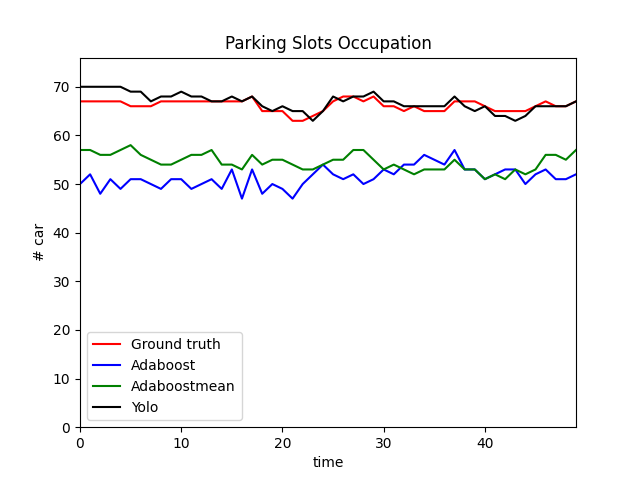
\includegraphics[width=0.5\textwidth]{pic/Parking_Slots_Occupation.png}
\end{figure}
\FloatBarrier
可以發現Yolo的Accuracy與Parking Slots Occupation表現都比Adaboost好,但使用mean當threshold表現上又比單純使用0當threshold的方法略好一些。
\section{Problem I meet}
\subsection{SelectBest}
當時在看完adaboost algorithm後卻不知道selectbest要我做甚麼,以及如何產出一堆的weekclassifier,原本以為是要我們做調整weight參數的部分,但又看到期已經在code內。產生weekclassifier的方法遠本也以為是用調整threshold,因為不知道Haarfeature在幹嘛。
\subsection{Yolov5}
Colab的路徑部分遇到了一些問題,在detect部分要讀檔的路徑問題。以及colab不能用waitkey,以及要我們replace clf.classify() with yolov5\_func.classify()但其實不能直接使用要在前面加上HW1\_material.。另外在在draw的部分不知為何沒有import pandas as pd。
\subsection{other}
Adaboost跑得很久,又要從T = 1跑到T = 10,其feature的算法似乎很暴力,每張圖會有13w左右的feature,總共又有600張圖
\section{Problem I solve}
\subsection{SelectBest}
最後用輸入輸出推出要使用每個feature去產生weekclassifier,並去大概看了一下featureVal在幹麻與其分布而有調整Threshold = mean的版本。
\subsection{Yolov5}
最後從上面的code與查了一下才找到路徑,draw的部分我直接copy下來本機跑,並多繪製了Threshold = mean 的摺線
\subsection{other}
後來有發現adaboost可以把CLF存下來,而且相同T取到的feature一樣(SelectBest回傳的一樣),最後只跑一次T = 10 並在每次存下當前T的CLF,想知道每次T的accuracy rate只要跑main.py內的utils.evaluate部分就好了(雖然發現時已經很晚了)
\begin{figure}[!ht]
    \centering
    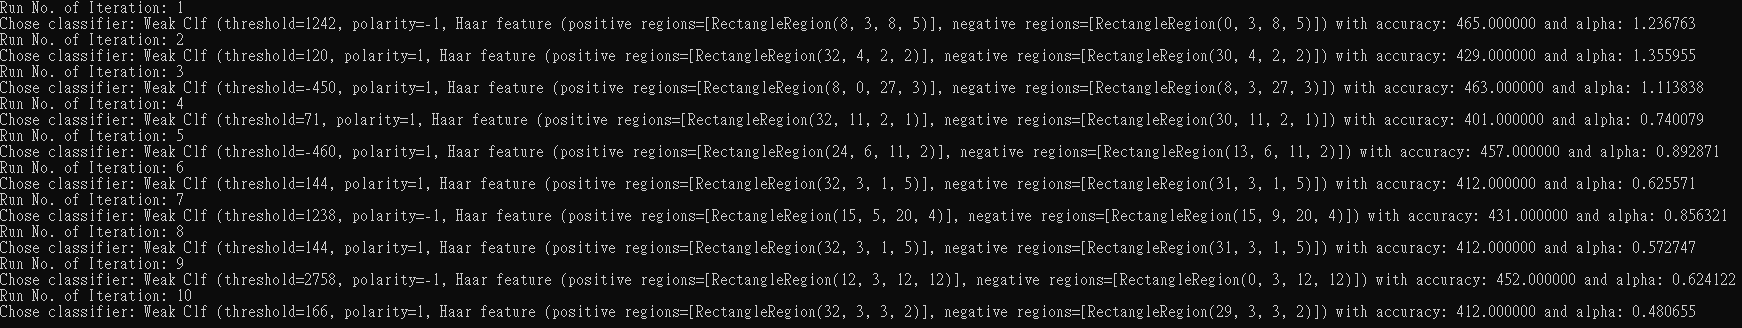
\includegraphics[width=0.8\textwidth]{pic/withmean/overview.png}
\end{figure}
\FloatBarrier
另外在執行時我把adaboost.py中buildfeatures內w與h調大產生較少的feature以加速測試,但其實調大一些雖然feature少了很多但正確沒下降多少
\subsection{New Problem}
\begin{itemize}
    \item 是否有更好取threshold的方法可以增進adaboost的表現(類似影像處理的Otsu Threshold,找featureval分布兩分布曲線的交界處)
    \item yolov5在本機執行,因為colab上路徑麻煩又要跑很久,不確定是否能直接弄下來在本機執行(GPU設定等)
    \item feature的數量選擇,能否調整w與h找到執行時間與accuracy的平衡點。
\end{itemize}
\section{Code}
Adaboost code can be find in\\
https://github.com/Sakuya0229/Artificial-Intelligence-HW1
\end{itemize}







\end{document}
